% XeLaTeX

\documentclass{article}
\usepackage{ctex}
\usepackage{xypic}
\usepackage{amsfonts,amssymb}
\usepackage{multirow}
\usepackage{geometry}
\usepackage{graphicx}
\usepackage{listings}
\usepackage{lipsum}
\usepackage{courier}
\usepackage{fancyvrb}
\usepackage{etoolbox}


\linespread{1.2}
\geometry{left=3cm,right=2.5cm,top=2.5cm,bottom=2.5cm}

\makeatletter
\patchcmd{\FV@SetupFont}
  {\FV@BaseLineStretch}
  {\fontencoding{T1}\FV@BaseLineStretch}
  {}{}
\makeatother

\lstset{basicstyle=\small\fontencoding{T1}\ttfamily,breaklines=true}
\lstset{numbers=left,frame=shadowbox,tabsize=4}
%\lstset{extendedchars=false}
\begin{document}

\title{实验十 \text{ } 计数、译码、显示综合实验 \text{ } 实验报告}
\author {16337233 王凯祺}
\maketitle

\section{实验目的}

熟悉中规模集成电路计数器的功能及应用

熟悉中规模集成电路译码器的功能及应用

熟悉LED数码管及显示电路的工作原理

\section{实验仪器}

1. 实验箱、万用表、示波器

2. 74LS160、74LS48、74LS00、74LS20

\section{实验内容}

用 74LS160 设计 60 进制计数器

\subsection{同步置数}

将 5 和 9 的二进制表示中 1 的位置通过与非门,接到置数端。置数输入全为 0 。

\begin{figure}[!hbp]
  \centering
  \includegraphics[scale=0.45]{ds.png}
\end{figure}

上图中, $D_0$ 表示时钟, $D_1 \cdots D_4$ 表示十位从高位到低位的二进制数, $D_5 \cdots D_8$ 表示个位从高位到低位的二进制数。

\subsection{异步清零}

将 6 的二进制表示中 1 的位置通过与非门,接到清零端。如下图。

\begin{figure}[!hbp]
  \centering
  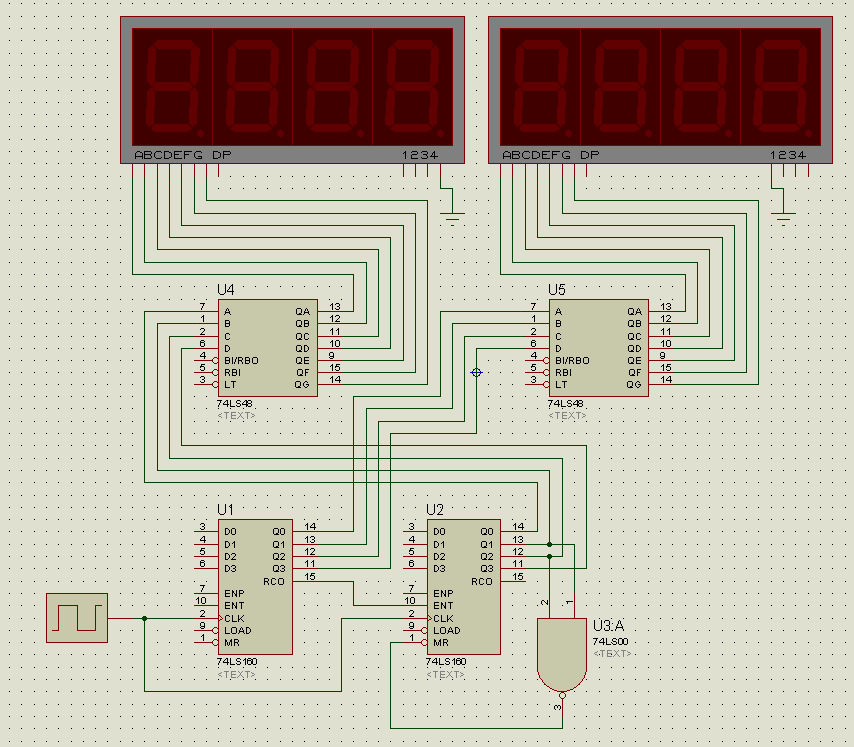
\includegraphics[scale=0.5]{ss.png}
\end{figure}

\end{document}
















